% Created 2018-07-11 Wed 15:37
% Intended LaTeX compiler: pdflatex
\documentclass[11pt]{article}
\usepackage[utf8]{inputenc}
\usepackage[T1]{fontenc}
\usepackage{graphicx}
\usepackage{grffile}
\usepackage{longtable}
\usepackage{wrapfig}
\usepackage{rotating}
\usepackage[normalem]{ulem}
\usepackage{amsmath}
\usepackage{textcomp}
\usepackage{amssymb}
\usepackage{capt-of}
\usepackage{hyperref}
\usepackage{placeins}
\usepackage[margin=0.5in]{geometry}
\usepackage[parfill]{parskip}
\date{\today}
\title{}
\hypersetup{
 pdfauthor={},
 pdftitle={},
 pdfkeywords={},
 pdfsubject={},
 pdfcreator={Emacs 26.0.91 (Org mode 9.1.13)}, 
 pdflang={English}}
\begin{document}

\tableofcontents

\section{Ressourcen, Prozesse und Ziele betrieblicher Leistungserstellung}
\label{sec:org03466ae}
\subsection{Leistungsbereich(Produktion)}
\label{sec:org6ad50d4}
\begin{center}
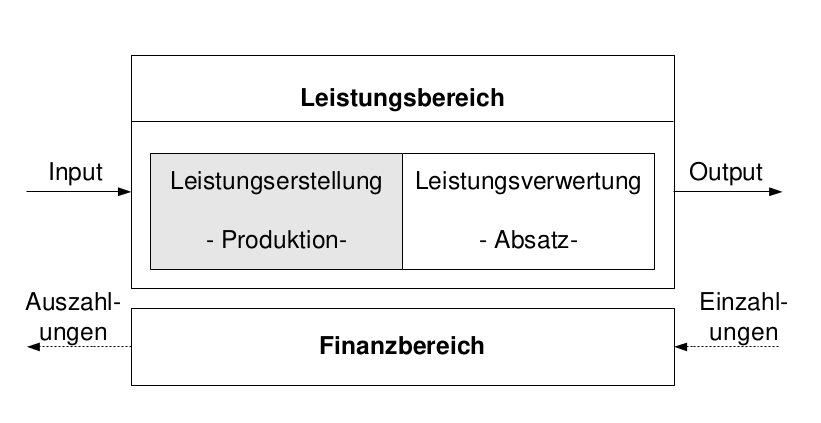
\includegraphics[width=250px]{./pictures/leistungsbereich_prod.png}
\end{center} 

\subsubsection{Produktion, Produktionsfaktoren, Produktionswirtschaft}
\label{sec:orgf2760ba}
\textbf{Produktion} = der industrielle Abbau von Material, dessen Be- und Verarbeitung und die Ausführung von Dienstleistungen; ist die methodische Umwandlung von Produktionsfaktoren in Produkte im Rahmen von bestimmten Produktionsverfahren

\textbf{Produktionsfaktoren} = sind die in der Produktion eingesetzen materiellen und immateriellen Güter, durch deren Gebrauch \& Verbrauch neue Sachgüter \& Dienstleistungen (Services) entsehen; Produktionsmittel nach Gutenberg = Betriebsmittel, Werkstoffe, (objektbezogene/dispositive) Arbeitsleistungen

\textbf{Produktionswirtschaft} = Aufgabe der Produktionswirtschaft ist die Planung, Durchführung \& Kontrolle der industriellen Leistungserstellung, um wirtschaftliche Produktionsstrukturen zu erreichen \& zu sichern
\subsection{Finanzierungsbereich}
\label{sec:orgf999c27}

\begin{center}
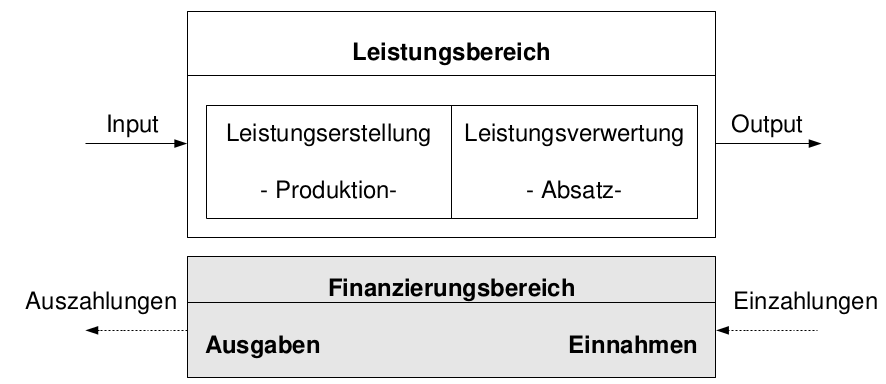
\includegraphics[width=250px]{./pictures/finanzierungsbereich.png}
\end{center} 

Finanzierung ist sowas wie eine Beanspruchung unter Versprechen auf Erfüllung
\begin{itemize}
\item betriebliche Finanzierung umfasst Beschaffung und Rückzahlung finanzieller Mittel und damit verbunden die Gestaltung der Beziehungen zw Unternehmen und Kapitalgebern
\item \emph{Finanzierungsmaßnahmen} beginnen mit Einzahlung an das Unternehmen, worauf Auszahlungen in späteren Perioden Folgen (Passivseite der Bilanz)
\item Gesamtheit aller Finanzmittel eines Unternehmens wird als Kapital bezeichnet
\end{itemize}

Investition ist sowas wie Verzicht in der Hoffnung auf Belohnung
\begin{itemize}
\item zielgerichteter Einsatz von finanziellen Mitteln zur Erwirtschaftung von Erträgen
\item \emph{Investitionsmaßnahmen} beginnen mit Auszahlung an das Unternehmen, auf die Einzahlungen in späteren Perioden folgen (Aktivseite der Bilanz)
\end{itemize}

\subsubsection{Finanzwirtschaft \& Zahlungsströme}
\label{sec:org0c3a73a}
\textbf{Monetärer Kapitalbegriff} = im Unternehmen eingesetzte Zahlungsmittel

\textbf{Finanzierung} ist die Kapitalbeschaffung für die jeweilige Unternehmung. Die \textbf{Finanzwirtschaft} umfasst diese Kapitalbeschaffung und -verwendung in der Unternehmung. Zu den finanzwirtschaftlichen Zielen gehört die Erreichung eines \emph{finanzwirtschaftlichen Gleichgewichts}, das bedeutet die Sicherung der dispositiven Liquidität, sowie die Sicherung der strukturellen Liquidität.

Die Funktion des \textbf{Finanzmanagements} ist die zielgerichtete Gestaltung der betrieblichen Finanzwirtschaft. Dazu zählt hauptsächlich die aktive Gestaltung der Kapitalzuführung \& des Kapitalentzugs.

\paragraph{Monetäre Zielgrößen}
\begin{itemize}
\item Zahlungsmittelbestand = Kassenbestand, Guthaben bei Kreditinstituren; Einzahlung, Auszahlung
\item Geldvermögen = Zahlungsmittelbestand + Forderungen - Verbindlichkeiten; Einnahme, Ausgabe
\item Gesamtvermögen = Gewinn + Verlustrechnung; Ertrag, Aufwand
\item Betriebsnotwendiges Vermögen = Kosten- und Leistungsrechnung; Ertrag, Aufwand
\end{itemize}

\section{Ressourcenbereitstellung \& Wettbewerbsfähigkeit}
\label{sec:org54e8953}
\subsection{Gegenstandbereich \& Ziele betrieblicher Leistungserstellung}
\label{sec:orgacd164a}
\subsubsection{Betriebliche Leistungserstellung als Kombinationsprozess}
\label{sec:orgda8517e}
"\emph{Die Ergiebigkeit des Faktoreinsatzes in den  Betrieben ist einmal von der Beschaffenheit der Faktoren selbst und zum anderen von ihrer Kombination abhängig.
Es gilt deshalb zu untersuchen, welche Umstände es sind, die den produktiven Beitrag bestimmen, den sie im Rahmen einer Faktorkombination zu leisten imstande sind.}" (Gutenberg 1975)

Beim Input der betrieblichen Leistungserstellung unterscheidet man zwischen Potential- und Repetierfaktoren
\begin{center}
\begin{tabular}{ll}
 & Repetierfaktoren (Verbrauch)\\
Charakteristik & gehen im Produktionsprozess physisch \& mengenmäßig unter\\
Bestimmung des Werteverzehrs & i.d.R leicht zu bewerten \& zuzuordnen\\
Teilbarkeit & i.d.R beliebig teilbar\\
Beispiele & Werkstoffe, Energie\\
\end{tabular}
\end{center}

\begin{center}
\begin{tabular}{ll}
 & Potentialfaktoren (Gebrauch/Bestand)\\
Charakteristik & stellen längerfristig verfügbare Nutzungspotentiale bereit\\
Bestimmung des Werteverzehrs & schwer bestimmtbar, Unsicher in der Zuordnung zB technischer Verschleiß\\
Teilbarkeit & i.d.R nicht beliebig teilbar\\
Beispiele & materiell: maschinelle Anlagen, Gebäude; immateriell: Rechte (Patente, Lizenzen), technische Informationen (Software)\\
\end{tabular}
\end{center}

\begin{figure}[htbp]
\centering
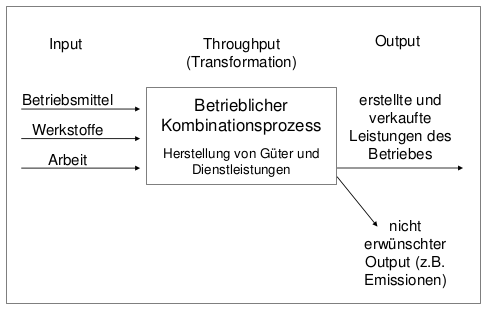
\includegraphics[width=250px]{./pictures/produktion_als_kombpr.png}
\caption{Produktion als Kombinationsprozess}
\end{figure} 

\(\rightarrow\) Ziele in dem obgigen Kombinationsprozess:
Beim Input ist die Verbesserung des Faktoreinsatzes, also eine Erhöhung der Produktivität das Ziel.
In der Transformation bzw dem Throughput ist eine Steigerung der Ausbringungsmenge bzw eine maximale Kapazitätsauslastung, sowie eine Verkürzung der Durchlauf- oder Produktionszeiten und eine Minimierung der Produktionskosten das Ziel.
Im Output wird die Steigerung des Qualitätsniveaus + der Zuverlässigkeit, sowie die Verbesserung der Arbeitsbedingungen oder des Umweltschutzes als Ziel anvisiert.

\subsubsection{Ziele \& Zielkonflikte produktionswirtschaftlicher Betätigung}
\label{sec:orgbf63e66}
\begin{enumerate}
\item Inhaltliche Ziele \& Zielkonflikte
\label{sec:org851d0d2}
Man kann inhatlich zwischen dem Werziel Produktivität, dem Humanziel Flexibilität und dem Sachziel Qualität unterscheiden. Die Ziehlbeziehungen dieser Ziele sind indifferent, komplementär und/oder konkurrierend.

\begin{figure}[htbp]
\centering
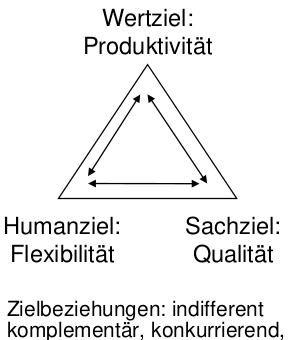
\includegraphics[width=250px]{./pictures/inhaltziele.png}
\caption{Inhaltliche Zielbeziehungen}
\end{figure} 

\item Unternehmensbeteiligte \& Interessenkonflikte
\label{sec:org0fe2736}
Innerhalb des Unternehmens kann es zu diversen Konflikten \& Spannung zwischen den verschiedenen Beteiligten kommen.

Ziele/Interessen der jeweiligen Unternehmensbeteiligten:
\begin{itemize}
\item Kapitalgeber: Rentabilität des eingesetzten Kapitals
\item Mitarbeiter: ihrem Leistungsbeitrag entsprechende Anreizstrukturen (Entlohnung)
\item Lieferanten/Kunden: Absatzsicherheit, Liefersicherheit, Qualität und Liquidität
\item Öffentlichkeit: Nachhaltigkeit, Transparenz
\end{itemize}

\item Sachliche Ziele produktionswirtschaftlicher Betätigung
\label{sec:org78d8e7e}

\textbf{\textbf{Produktionsziele}}:
Aus dem produktionswirtschaftlichen Sachziel der Herstellung von Gütern und/oder Dienstleistungen nach Mengen-, Zeit- und Qualitätskriterien leiten sich die
produktionswirtschaftlichen Teilziele ab.
\begin{itemize}
\item Bestimmung von Anspruchsniveaus
\item Abbildung von Wirkungszusammenhängen
\end{itemize}

\textbf{\textbf{Produktionsstrategien}}:
Das Produktionssystem wird durch strategische Maßnahmen in die Lage versetzt, seine Potenziale so aufzubauen, dass sie den zukünftig auftretenden Anforderungen gerecht werden (SWOT-Analyse).

\textbf{\textbf{Produktionspolitik}}:
Die auf die Produktionsebene "heruntergebrochenen" Ziele des Unternehmens finden in der Produktionspolitik ihre Gestaltungs- und Entscheidungsmodelle
\end{enumerate}
\subsection{Ressourcenbereitstellung als nachhaltiger Wettbewerbsvorteil}
\label{sec:org24625fb}
\subsubsection{Produktionssysteme(-verfahren)}
\label{sec:org5efcd7a}
In einer gegebenen Situation wird aus allen möglichen Produkten \& Dienstleistungen ein \textbf{Produktionsprogramm} zusammengesetzt (Zielfunktion). Bei der betriebswirtschaftlichen Analyse des Produktionsprozesses sind alle Situationen \& Veränderungsmöglichkeiten zu betrachten, die auf die Zielfunktion und die Nebenbedingungen einwirken.

Das \textbf{Produktionsverfahren} bezeichnet die organisatorische \& technologische Art, in welcher ein Betrieb Produktionsfaktoren kombinieren und wie er diesen Prozess durchführt.

\subsubsection{Produktionsfunktion und Produktionsmodelle}
\label{sec:orgd8fa659}
\begin{center}
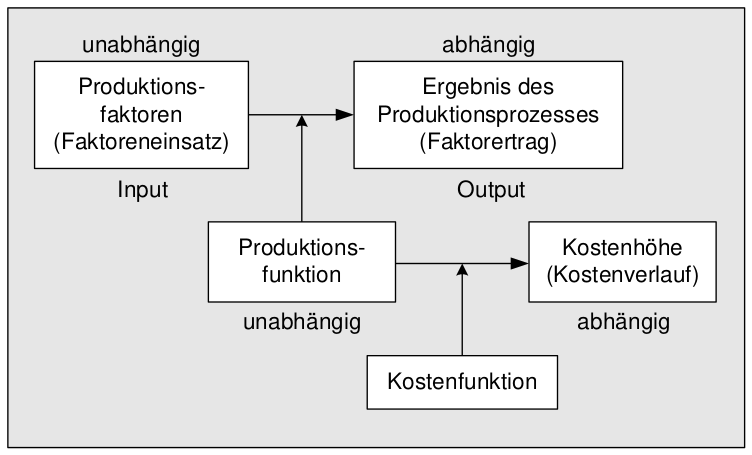
\includegraphics[width=250px]{./pictures/prodfunktion.png}
\end{center} 

Beispiel einer Produktionsfunktion: \(x=f(r_1, r_2, r_3)\)

\textbf{Kombinationsprinzip}:\\
Zur betrieblichen Leistungserstellung in einer Periode \(x\) (= Ausbringungsmenge/Output) sind alle drei Einsatzfaktoren (resources) \(r_1\) (= Verbrauch Werkstoff/Menge), \(r_2\) (= Einsaz Arbeitsstunden), \(r_3\) (= Einsatz Maschinenstunden) notwendig. Ist einer dieser Faktoren nicht vorhanden, kommt keine Leistungserstellung zustande.

\textbf{Faktorproportionsprinzip}:\\
Die Wahl der Faktorkombination \(f\) bestimmt das Verhältnis, indem die drei Faktoren miteinander kombiniert werden.

\textbf{Effizienzprinzip}:\\
Die Menge der Produktionsfaktoren, die zur Herstellung von \(x\) notwendig ist, wird bei gegebener Produktionsfunktion \(f\) genau bestimmt. Mit einem geringeren Faktorverbrauch kann \(x\) nicht hergestellt werden. Werden mehr Faktoren verbraucht liegt Verschwendung vor.

\begin{enumerate}
\item Produktionstheoretische Grundbegriffe
\label{sec:orgc947267}
\begin{itemize}
\item \textbf{Grenzrate der Faktorsubstitution} = Austauschrelation zwischen zwei Produktionsfaktoren \(r_1\) und \(r_2\) bei Konstanz der Ausbringungsmenge x
\item \textbf{Grenzproduktivität} = Veränderung der Ausbringungsmenge x in Abhängikeit von infinitisemal kleinen Änderungen der Faktoreinsatzmengen \(r_1\) bzw \(r_2\)
\item \textbf{Durchschnittsertrag} = Durchschnittlicher Ertrag des Produktionsfaktors \(r_1\) bzw \(r_2\)
\item \textbf{Produktionskoeffizient} = Anzahl der im Produktionsprozess durchschnittlich notwendigen Faktoreinsatzmengen \(r_1\) bzw \(r_2\) zur Produktion einer Einheit z
\end{itemize}

\item Kostenfunktion: Bewertung des Faktoreinsatzes
\label{sec:orgb58b3d3}
\$K = f(x)\$\\
\begin{itemize}
\item \textbf{Kosten/Gesamtkosten} = Die mit Preisen bewertete Faktoreinsatzmengen, die während einer Rechnungsperiode in Abhängikeit von dem Beschäftigungsgrad anfallen
\item \textbf{Kostenrate/Stückkosten} = Der Betrag der auf eine Leistungseinheit entfallenden Kosten (bei Angabe der Ausbringungsmenge in Stück)
\item \textbf{Grenzkosten} = Geben für jeden Beschäftigungsgrad x den Anstieg der Gesamtkostenkurve an
\item \textbf{Fixe Kosten} = Kosten der Betriebsbereitschaft, unabhängig von der tatsächlichen Leistung, zB Zinsen, Mieten, Abschreibungen
\begin{itemize}
\item Nutzkosten/Leerkosten = Abgrenzung der Kostenwirkungen der nicht beanspruchten Kapazitäten
\end{itemize}
\item \textbf{Variable Kosten} = Kosten in Abhängikeit von der tatsächlichen Leistung (proportionale, degressive, progressive Kostenverläufe)
\end{itemize}

\item Grundlegende Kritikpunkte
\label{sec:org8a559f5}
\begin{itemize}
\item mangelnde Untersuchung der Dynamik \& Unsicherheit des Produktionsgeschehens
\item ungenügende Einbeziehung der betrieblichen Organisationsstruktur
\item nicht ausreichende Berücksichtigung von Führungstätigkeiten
\item Beschränkung auf quantitative Größen
\item ungenügende Erfassung von Dienstleistungen
\item zu hohe Aggregation und zu geringe empirische Fundierung der verwendeten Größen
\end{itemize}
\end{enumerate}

\subsubsection{Produktionskonzepte und - strategien}
\label{sec:org2b34487}
\begin{itemize}
\item Qualitätsorientierung
\item Best-practive Orientierung
\item Lernende Organisation
\item Mitarbeiter-orientierte Prozesse
\item nicht imitierbare Ressourcen wie bswp Patente, besonders einzigartige Standpunkte oder Assets sind wertvollere Ressourcen als leicht imitierbare Ressourcen wie bspw Cash oder Rohstoffe \(\rightarrow\) Generierung nicht-imitierbarer Produktionsfähigkeiten
\item Identifikation oder Entwicklung geschützter Ressourcenpositionen
\end{itemize}
\end{document}
